\chapter{Recorrido de grafos}

En este capítulo discutiremos dos algoritmos de grafos
fundamentales: la búsqueda en profundidad y la búsqueda en anchura.
Los dos algoritmos reciben un nodo inicial en el grafo,
y visitan todos los otros nodos que sean alcanzables desde el
nodo inicial. La diferencia en los algoritmos es el orden
en que visitan los nodos.

\section{Búsqueda en profundidad}

\index{búsqueda en profundidad}

La \key{búsqueda en profundidad} (DFS, por \textit{depth-first search})
es una técnica de recorrido sencilla. El algoritmo comienza en el
nodo inicial, y procede a todos los nodos alcanzables usando aristas
del grafo.

La búsqueda en profundidad siempre sigue un solo camino en el grafo
mientras siga encontrado nuevos nodos. Luego de esto, vuelve
a nodos previos y comienza a explorar nuevos caminos del grafo.
El algoritmo mantiene un registro de nodos visitados, así procesa
cada nodo una sola vez.

\subsubsection*{Ejemplo}

Veamos cómo la búsqueda en profundidad procesa
el siguiente grafo:
\begin{center}
    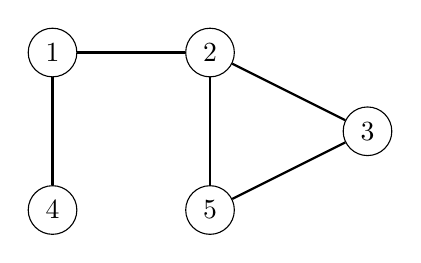
\begin{tikzpicture}
        \node[draw, circle] (1) at (1,5) {$1$};
        \node[draw, circle] (2) at (3,5) {$2$};
        \node[draw, circle] (3) at (5,4) {$3$};
        \node[draw, circle] (4) at (1,3) {$4$};
        \node[draw, circle] (5) at (3,3) {$5$};

        \path[draw,thick,-] (1) -- (2);
        \path[draw,thick,-] (2) -- (3);
        \path[draw,thick,-] (1) -- (4);
        \path[draw,thick,-] (3) -- (5);
        \path[draw,thick,-] (2) -- (5);
    \end{tikzpicture}
\end{center}
Podemos comenzar la búsqueda en cualquier nodo del grafo;
por ahora comencemos en el nodo 1.

La búsqueda primero procede al nodo 2:
\begin{center}
    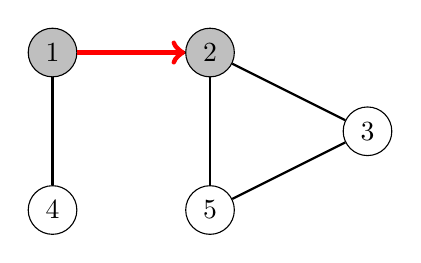
\begin{tikzpicture}
        \node[draw, circle,fill=lightgray] (1) at (1,5) {$1$};
        \node[draw, circle,fill=lightgray] (2) at (3,5) {$2$};
        \node[draw, circle] (3) at (5,4) {$3$};
        \node[draw, circle] (4) at (1,3) {$4$};
        \node[draw, circle] (5) at (3,3) {$5$};

        \path[draw,thick,-] (1) -- (2);
        \path[draw,thick,-] (2) -- (3);
        \path[draw,thick,-] (1) -- (4);
        \path[draw,thick,-] (3) -- (5);
        \path[draw,thick,-] (2) -- (5);

        \path[draw=red,thick,->,line width=2pt] (1) -- (2);
    \end{tikzpicture}
\end{center}
Luego de esto, se visitan los nodos 3 y 5:
\begin{center}
    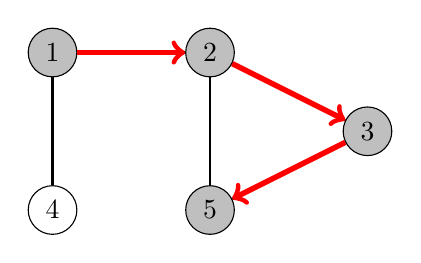
\begin{tikzpicture}
        \node[draw, circle,fill=lightgray] (1) at (1,5) {$1$};
        \node[draw, circle,fill=lightgray] (2) at (3,5) {$2$};
        \node[draw, circle,fill=lightgray] (3) at (5,4) {$3$};
        \node[draw, circle] (4) at (1,3) {$4$};
        \node[draw, circle,fill=lightgray] (5) at (3,3) {$5$};

        \path[draw,thick,-] (1) -- (2);
        \path[draw,thick,-] (2) -- (3);
        \path[draw,thick,-] (1) -- (4);
        \path[draw,thick,-] (3) -- (5);
        \path[draw,thick,-] (2) -- (5);

        \path[draw=red,thick,->,line width=2pt] (1) -- (2);
        \path[draw=red,thick,->,line width=2pt] (2) -- (3);
        \path[draw=red,thick,->,line width=2pt] (3) -- (5);
    \end{tikzpicture}
\end{center}
Los vecinos del nodo 5 son 2 y 3, pero ya
hemos visitado a los dos, así que es hora de volver
a nodos previos. También hemos visitado los vecinos de
nodos 3 y 2, por lo que nos movemos del nodo 1 al nodo 4:
\begin{center}
    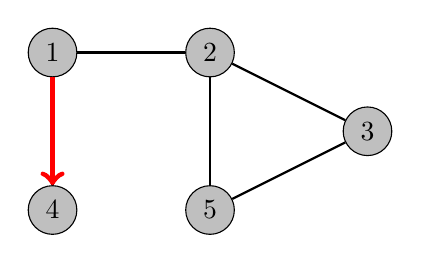
\begin{tikzpicture}
        \node[draw, circle,fill=lightgray] (1) at (1,5) {$1$};
        \node[draw, circle,fill=lightgray] (2) at (3,5) {$2$};
        \node[draw, circle,fill=lightgray] (3) at (5,4) {$3$};
        \node[draw, circle,fill=lightgray] (4) at (1,3) {$4$};
        \node[draw, circle,fill=lightgray] (5) at (3,3) {$5$};

        \path[draw,thick,-] (1) -- (2);
        \path[draw,thick,-] (2) -- (3);
        \path[draw,thick,-] (1) -- (4);
        \path[draw,thick,-] (3) -- (5);
        \path[draw,thick,-] (2) -- (5);

        \path[draw=red,thick,->,line width=2pt] (1) -- (4);
    \end{tikzpicture}
\end{center}
Luego de esto, la búsqueda termina porque ha visitado
todos los nodos.

La complejidad temporal de la búsqueda en profundidad es de $O(n+m)$
donde $n$ es la cantidad de nodos y $m$ la cantidad de aristas,
porque el algoritmo procesa cada nodo y arista una vez.

\subsubsection*{Implementación}

La búsqueda en profundidad puede implementarse convenientemente
usando recursión. La siguiente función \texttt{dfs} comienza una
búsqueda en profundidad en un nodo dado. La función asume que
el grafo está almacenado como listas de adyacencia en un arreglo
\begin{lstlisting}
vector<int> ady[N];
\end{lstlisting}
y a la vez mantiene un arreglo
\begin{lstlisting}
bool visitado[N];
\end{lstlisting}
que registra los nodos visitados.
Inicialmente, cada valor del arreglo es \texttt{false},
y cuando la búsqueda visita un nodo $s$,
el valor de \texttt{visitado}[$s$] se hace \texttt{true}.

La función puede implementarse de la siguiente manera:
\begin{lstlisting}
void dfs(int s) {
    if (visitado[s]) return;
    visitado[s] = true;
    // procesar nodo s
    for (auto v : ady[s]) {
        dfs(v);
    }
}
\end{lstlisting}

\section{Búsqueda en anchura}

\index{búsqueda en anchura}

La \key{búsqueda en anchura} (BFS, por \textit{breadth-first search})
visita todos los nodos en orden creciente de su distancia al
nodo inicial. Por lo tanto, podemos calcular la distancia del nodo
inicial a todos los otros nodos utilizando la búsqueda en anchura.
No obstante, este algoritmo es más difícil de implementar que la
búsqueda en profundidad.

La búsqueda en anchura visita los nodos un nivel tras otro.
Primero, explora los nodos a distancia 1 del nodo inicial,
luego los nodos a distancia 2, y así sucesivamente.
Este proceso continúa hasta que todos los nodos han sido visitados.

\subsubsection*{Ejemplo}

Veamos cómo la búsqueda en anchura procesa el siguiente grafo:
\begin{center}
    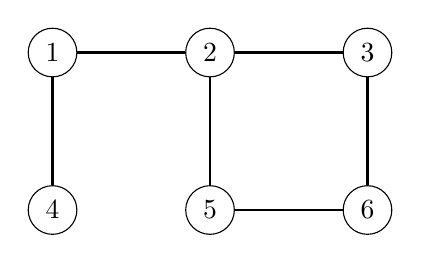
\begin{tikzpicture}
        \node[draw, circle] (1) at (1,5) {$1$};
        \node[draw, circle] (2) at (3,5) {$2$};
        \node[draw, circle] (3) at (5,5) {$3$};
        \node[draw, circle] (4) at (1,3) {$4$};
        \node[draw, circle] (5) at (3,3) {$5$};
        \node[draw, circle] (6) at (5,3) {$6$};

        \path[draw,thick,-] (1) -- (2);
        \path[draw,thick,-] (2) -- (3);
        \path[draw,thick,-] (1) -- (4);
        \path[draw,thick,-] (3) -- (6);
        \path[draw,thick,-] (2) -- (5);
        \path[draw,thick,-] (5) -- (6);
    \end{tikzpicture}
\end{center}

Supongamos que la búsqueda comienza en el nodo 1. Primero,
procesaremos todos los nodos que sean alcanzables desde el nodo 1
utilizando una sola arista:
\begin{center}
    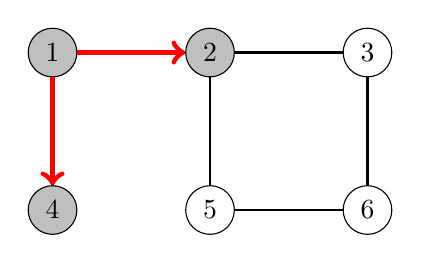
\begin{tikzpicture}
        \node[draw, circle,fill=lightgray] (1) at (1,5) {$1$};
        \node[draw, circle,fill=lightgray] (2) at (3,5) {$2$};
        \node[draw, circle] (3) at (5,5) {$3$};
        \node[draw, circle,fill=lightgray] (4) at (1,3) {$4$};
        \node[draw, circle] (5) at (3,3) {$5$};
        \node[draw, circle] (6) at (5,3) {$6$};

        \path[draw,thick,-] (1) -- (2);
        \path[draw,thick,-] (2) -- (3);
        \path[draw,thick,-] (1) -- (4);
        \path[draw,thick,-] (3) -- (6);
        \path[draw,thick,-] (2) -- (5);
        \path[draw,thick,-] (5) -- (6);

        \path[draw,thick,-] (1) -- (2);
        \path[draw,thick,-] (2) -- (3);
        \path[draw,thick,-] (1) -- (4);
        \path[draw,thick,-] (2) -- (5);

        \path[draw=red,thick,->,line width=2pt] (1) -- (2);
        \path[draw=red,thick,->,line width=2pt] (1) -- (4);
    \end{tikzpicture}
\end{center}

Luego de esto, procedemos a los nodos 3 y 5:
\begin{center}
    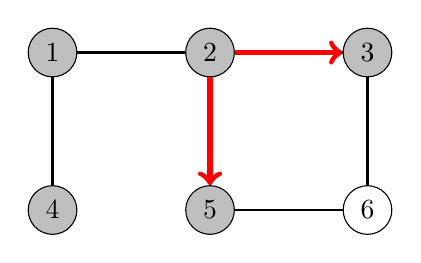
\begin{tikzpicture}
        \node[draw, circle,fill=lightgray] (1) at (1,5) {$1$};
        \node[draw, circle,fill=lightgray] (2) at (3,5) {$2$};
        \node[draw, circle,fill=lightgray] (3) at (5,5) {$3$};
        \node[draw, circle,fill=lightgray] (4) at (1,3) {$4$};
        \node[draw, circle,fill=lightgray] (5) at (3,3) {$5$};
        \node[draw, circle] (6) at (5,3) {$6$};

        \path[draw,thick,-] (1) -- (2);
        \path[draw,thick,-] (2) -- (3);
        \path[draw,thick,-] (1) -- (4);
        \path[draw,thick,-] (3) -- (6);
        \path[draw,thick,-] (2) -- (5);
        \path[draw,thick,-] (5) -- (6);

        \path[draw,thick,-] (1) -- (2);
        \path[draw,thick,-] (2) -- (3);
        \path[draw,thick,-] (1) -- (4);
        \path[draw,thick,-] (2) -- (5);

        \path[draw=red,thick,->,line width=2pt] (2) -- (3);
        \path[draw=red,thick,->,line width=2pt] (2) -- (5);
    \end{tikzpicture}
\end{center}

Finalmente, visitamos el nodo 6:
\begin{center}
    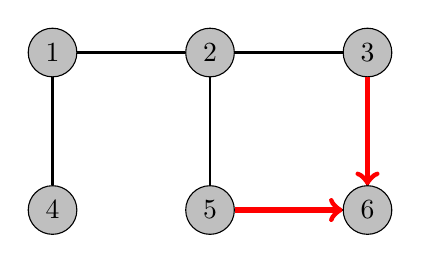
\begin{tikzpicture}
        \node[draw, circle,fill=lightgray] (1) at (1,5) {$1$};
        \node[draw, circle,fill=lightgray] (2) at (3,5) {$2$};
        \node[draw, circle,fill=lightgray] (3) at (5,5) {$3$};
        \node[draw, circle,fill=lightgray] (4) at (1,3) {$4$};
        \node[draw, circle,fill=lightgray] (5) at (3,3) {$5$};
        \node[draw, circle,fill=lightgray] (6) at (5,3) {$6$};

        \path[draw,thick,-] (1) -- (2);
        \path[draw,thick,-] (2) -- (3);
        \path[draw,thick,-] (1) -- (4);
        \path[draw,thick,-] (3) -- (6);
        \path[draw,thick,-] (2) -- (5);
        \path[draw,thick,-] (5) -- (6);

        \path[draw,thick,-] (1) -- (2);
        \path[draw,thick,-] (2) -- (3);
        \path[draw,thick,-] (1) -- (4);
        \path[draw,thick,-] (2) -- (5);

        \path[draw=red,thick,->,line width=2pt] (3) -- (6);
        \path[draw=red,thick,->,line width=2pt] (5) -- (6);
    \end{tikzpicture}
\end{center}

Ahora hemos calculado las distancias desde el nodo inicial
a todos los otros nodos del grafo. Las distancias son
las siguientes:

\begin{center}
    \begin{tabular}{ll}
        \\
        nodo & distancia \\
        \hline
        1    & 0         \\
        2    & 1         \\
        3    & 2         \\
        4    & 1         \\
        5    & 2         \\
        6    & 3         \\
        \\
    \end{tabular}
\end{center}

Así como en la búsqueda en profundidad, la complejidad
de la búsqueda en anchura es $O(n+m)$, donde $n$ es el
número de nodos y $m$ es el número de aristas.

\subsubsection*{Implementación}

La búsqueda en anchura es más difícil de implementar que
la búsqueda en profundidad, porque el algoritmo visita nodos
en diferentes partes del grafo. Una implementación típica se
basa en una cola que contiene nodos. En cada paso, el siguiente
nodo de la cola será procesado.

El siguiente código asume que el grafo está almacenado
en listas de adyacencia y mantiene las siguientes estructuras:
\begin{lstlisting}
queue<int> cola;
bool visitado[N];
int distancia[N];
\end{lstlisting}

La \texttt{cola} contiene nodos a ser procesados en orden
creciente de su distancia. Los nuevos nodos siempre son añadidos al
final de la cola, y el nodo al principio de la cola es el siguiente
a ser procesado. El arreglo \texttt{visitado} indica cuáles nodos han
sido visitados, y el arreglo \texttt{distancia} contendrá las distancias
desde el nodo inicial a todos los nodos del grafo.

La búsqueda puede implementarse de la siguiente manera,
comenzando en el nodo $x$:
\begin{lstlisting}
visitado[x] = true;
distancia[x] = 0;
q.push(x);
while (!q.empty()) {
    int s = q.front(); q.pop();
    // procesar nodo s
    for (auto v : ady[s]) {
        if (visitado[v]) continue;
        visitado[u] = true;
        distancia[u] = distancia[s] + 1;
        q.push(u);
    }
}
\end{lstlisting}

\section{Aplicaciones}

Usando estos algoritmos de recorrido, podemos
revisar muchas propiedades de los grafos. Usualmente, cualquiera
de los dos algoritmos puede ser utilizado, pero en práctica, la
búsqueda en profundidad es una mejor opción por su facilidad de
implementación. En las siguientes aplicaciones asumiremos que el
grafo no es dirigido.

\subsubsection{Conectividad}

\index{grafo!conexo}

Un grafo es conexo si hay un camino desde cualquier
par de nodos en el grafo. Por ende, podemos revisar si un grafo
es conexo comenzando una búsqueda en cualquier nodo y revisando
si podemos alcanzar todos los otros nodos.

Por ejemplo, en el grafo
\begin{center}
    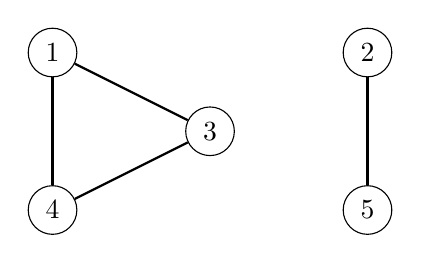
\begin{tikzpicture}
        \node[draw, circle] (2) at (7,5) {$2$};
        \node[draw, circle] (1) at (3,5) {$1$};
        \node[draw, circle] (3) at (5,4) {$3$};
        \node[draw, circle] (5) at (7,3) {$5$};
        \node[draw, circle] (4) at (3,3) {$4$};

        \path[draw,thick,-] (1) -- (3);
        \path[draw,thick,-] (1) -- (4);
        \path[draw,thick,-] (3) -- (4);
        \path[draw,thick,-] (2) -- (5);
    \end{tikzpicture}
\end{center}
una búsqueda en profundidad desde el nodo $1$ visita
los siguientes nodos:
\begin{center}
    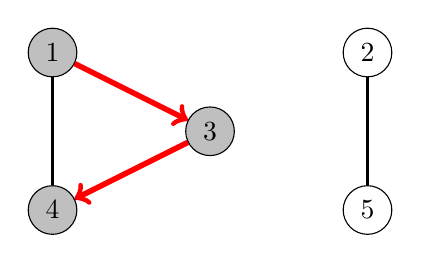
\begin{tikzpicture}
        \node[draw, circle] (2) at (7,5) {$2$};
        \node[draw, circle,fill=lightgray] (1) at (3,5) {$1$};
        \node[draw, circle,fill=lightgray] (3) at (5,4) {$3$};
        \node[draw, circle] (5) at (7,3) {$5$};
        \node[draw, circle,fill=lightgray] (4) at (3,3) {$4$};

        \path[draw,thick,-] (1) -- (3);
        \path[draw,thick,-] (1) -- (4);
        \path[draw,thick,-] (3) -- (4);
        \path[draw,thick,-] (2) -- (5);

        \path[draw=red,thick,->,line width=2pt] (1) -- (3);
        \path[draw=red,thick,->,line width=2pt] (3) -- (4);

    \end{tikzpicture}
\end{center}

Ya que la búsqueda no visitó todos los nodos, podemos
concluir que el grafo no es conexo. Similarmente,
también podemos encontrar todos los componentes conexos
de un grafo si iteramos a través de los nodos y comenzamos
una nueva búsqueda en profundidad siempre y cuando el nodo
todavía no haya sido visitado.

\subsubsection{Encontrar ciclos}

\index{ciclo}

Un grafo contiene un ciclo si, durante un recorrido,
encontramos un nodo cuyo vecino (aparte del previo nodo en
nuestro camino) ya ha sido visitado. Por ejemplo, el grafo
\begin{center}
    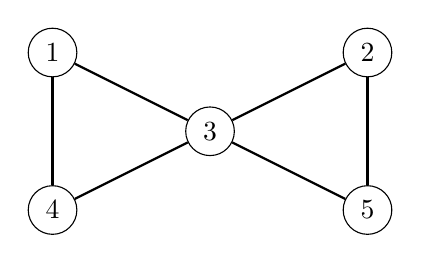
\begin{tikzpicture}
        \node[draw, circle] (2) at (7,5) {$2$};
        \node[draw, circle] (1) at (3,5) {$1$};
        \node[draw, circle] (3) at (5,4) {$3$};
        \node[draw, circle] (5) at (7,3) {$5$};
        \node[draw, circle] (4) at (3,3) {$4$};

        \path[draw,thick,-] (1) -- (3);
        \path[draw,thick,-] (1) -- (4);
        \path[draw,thick,-] (3) -- (4);
        \path[draw,thick,-] (2) -- (5);
        \path[draw,thick,-] (2) -- (3);
        \path[draw,thick,-] (3) -- (5);
    \end{tikzpicture}
\end{center}
contiene dos ciclos, y podemos encontrar uno
de ellos de la siguiente forma:
\begin{center}
    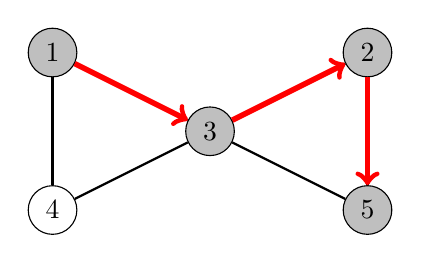
\begin{tikzpicture}
        \node[draw, circle,fill=lightgray] (2) at (7,5) {$2$};
        \node[draw, circle,fill=lightgray] (1) at (3,5) {$1$};
        \node[draw, circle,fill=lightgray] (3) at (5,4) {$3$};
        \node[draw, circle,fill=lightgray] (5) at (7,3) {$5$};
        \node[draw, circle] (4) at (3,3) {$4$};

        \path[draw,thick,-] (1) -- (3);
        \path[draw,thick,-] (1) -- (4);
        \path[draw,thick,-] (3) -- (4);
        \path[draw,thick,-] (2) -- (5);
        \path[draw,thick,-] (2) -- (3);
        \path[draw,thick,-] (3) -- (5);

        \path[draw=red,thick,->,line width=2pt] (1) -- (3);
        \path[draw=red,thick,->,line width=2pt] (3) -- (2);
        \path[draw=red,thick,->,line width=2pt] (2) -- (5);

    \end{tikzpicture}
\end{center}

Luego de movernos del nodo 2 al nodo 5, nos damos cuenta
de que el vecino 3 del nodo 5 ya ha sido visitado. Por
lo tanto, el grafo contiene un ciclo que pasa por el nodo 3,
por ejemplo, $3 \rightarrow 2 \rightarrow 5 \rightarrow 3$.

Otra forma de revisar si un grafo contiene un ciclo es
simplemente calcular el número de nodos y aristas en cada
componente. Si un componente contiene $c$ nodos y es acíclico,
debe contener exactamente $c-1$ aristas (debe ser un árbol).
Si hay $c$ o más aristas, el componente debe contener un ciclo.

\subsubsection{Bipartidismo}

\index{grafo!bipartito}

Un grafo es bipartito si sus nodos pueden ser coloreados
usando dos colores de tal forma que no haya dos nodos adyacentes
con el mismo color. Es sorprendentemente fácil revisar si un
grafo es bipartito utilizando algoritmos de búsqueda.

La idea es colorear el nodo inicial de azul, todos sus vecinos
de rojo, todos sus vecinos de azul, y así. Si en algún punto de la
búsqueda nos damos cuenta que dos nodos adyacentes tienen el mismo
color, esto significa que el grafo no es bipartito. De lo contrario
el grafo es bipartito y hemos encontrado una coloración.

Por ejemplo, el grafo
\begin{center}
    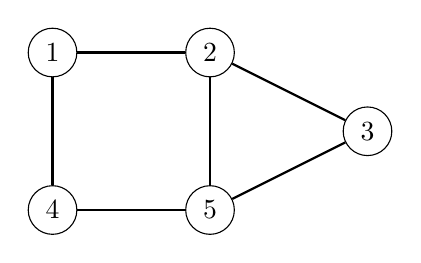
\begin{tikzpicture}
        \node[draw, circle] (2) at (5,5) {$2$};
        \node[draw, circle] (1) at (3,5) {$1$};
        \node[draw, circle] (3) at (7,4) {$3$};
        \node[draw, circle] (5) at (5,3) {$5$};
        \node[draw, circle] (4) at (3,3) {$4$};

        \path[draw,thick,-] (1) -- (2);
        \path[draw,thick,-] (2) -- (5);
        \path[draw,thick,-] (5) -- (4);
        \path[draw,thick,-] (4) -- (1);
        \path[draw,thick,-] (2) -- (3);
        \path[draw,thick,-] (5) -- (3);
    \end{tikzpicture}
\end{center}
no es bipartito, porque una búsqueda del nodo 1 procede
de la siguiente manera:
\begin{center}
    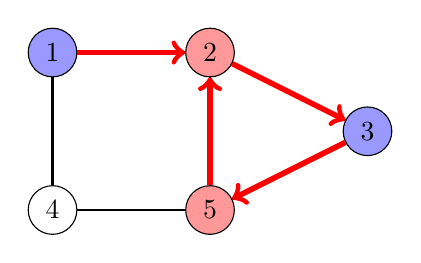
\begin{tikzpicture}
        \node[draw, circle,fill=red!40] (2) at (5,5) {$2$};
        \node[draw, circle,fill=blue!40] (1) at (3,5) {$1$};
        \node[draw, circle,fill=blue!40] (3) at (7,4) {$3$};
        \node[draw, circle,fill=red!40] (5) at (5,3) {$5$};
        \node[draw, circle] (4) at (3,3) {$4$};

        \path[draw,thick,-] (1) -- (2);
        \path[draw,thick,-] (2) -- (5);
        \path[draw,thick,-] (5) -- (4);
        \path[draw,thick,-] (4) -- (1);
        \path[draw,thick,-] (2) -- (3);
        \path[draw,thick,-] (5) -- (3);

        \path[draw=red,thick,->,line width=2pt] (1) -- (2);
        \path[draw=red,thick,->,line width=2pt] (2) -- (3);
        \path[draw=red,thick,->,line width=2pt] (3) -- (5);
        \path[draw=red,thick,->,line width=2pt] (5) -- (2);
    \end{tikzpicture}
\end{center}

Nos damos cuenta que el color de los nodos 2 y 5 es rojo
mientras que son adyacentes en el grafo. Por ende, el grafo no
es bipartito.

Este algoritmo siempre funciona, porque cuando hay solo dos
colores disponibles, el color del nodo inicial en un componente
determina los colores de todos los otros nodos en él.

Ten en cuenta que en el caso general, es difícil revisar si
los nodos de un grafo pueden ser coloreados usando $k$ colores
tal que no haya nodos adyacentes del mismo color. Incluso cuando
$k=3$, no existe un algoritmo eficiente y el problema es NP-difícil.